\problemname{Young Diagram}

\begin{figure}[!h]
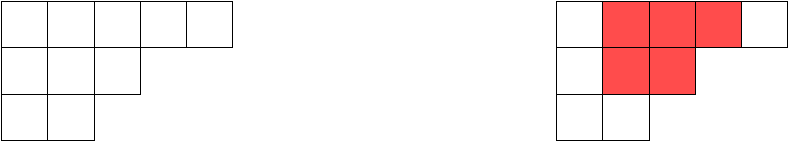
\includegraphics[width=0.98\textwidth]{young}
\caption{On the left, the Young diagram corresponding to the partition 10=5+3+2 is shown. On the right, it is demonstrated that the diagram for 10=5+3+2 (black outlines) can enclose the diagram for 5=3+2 (filled squares). On the other hand, the diagram for 10=5+3+2 cannot enclose the diagram for 8=4+4.}
\end{figure}

A \emph{Young diagram} is a way to visualize a partition of a positive integer $n$ into one or more integer terms:

$$n = m_1 + m_2 + ... + m_k$$

The diagram consists of $k$ rows with $m_i$ squares in each row (see the figure above). The rows are left-justified and always sorted by length so that the top row represents the largest term, and so on. A given row is thus either shorter than the row above it or of equal length. Sometimes one Young diagram can \emph{enclose} another. We say that diagram X can enclose diagram Y if it is possible to place diagram Y, without rotating or mirroring it, completely inside diagram X, i.e. so that every square in Y coincides with a square in X.

Write a program that, given an integer $n$, finds the partition of $n$ whose Young diagram can enclose the largest number of different Young diagrams.

\section*{Input}
The input consists of the integer $n$ ($1 \le n \le 100$).

\section*{Output}
Output an integer: the maximum number of Young diagrams that any single Young diagram with $n$ squares can enclose.
Then output a line with one or more positive integers, the number of squares in each row of this optimal diagram,
starting from the top. If there are multiple optimal diagrams, you may output any of them.

\section*{Scoring}
Your solution will be tested on a set of test groups.
To earn points for a group, you must pass all test cases in that group.

\noindent
\begin{tabular}{| l | l | p{12cm} |}
  \hline
  \textbf{Group} & \textbf{Points} & \textbf{Constraints} \\ \hline
  $1$    & $10$       & $n \leq 10$ \\ \hline
  $2$    & $25$       & $n \leq 20$ \\ \hline
  $3$    & $25$       & $n \leq 60$ \\ \hline
  $4$    & $40$       & No additional constraints. \\ \hline
\end{tabular}
